\documentclass[10pt]{report}
\usepackage{times}
\usepackage{anysize}
\usepackage{multicol}
\usepackage{fancyhdr}
\usepackage{graphicx}
\usepackage{amsmath}

\setlength{\headheight}{15.2pt}
\setlength{\headwidth}{495pt}
\setlength{\parindent}{0pt}
\setlength{\parskip}{1em}
\pagestyle{fancy}
\rhead{Page \thepage}
\lhead{COMP3130 Othello Project}
\marginsize{2cm}{1.5cm}{2cm}{2cm}

\newenvironment{packed_enum}{
\begin{enumerate}
  \setlength{\itemsep}{0pt}
  \setlength{\parskip}{0pt}
  \setlength{\parsep}{0pt}
}{\end{enumerate}}

\begin{document}

\date{June 8th, 2012}
\title{Team Reverwesome: Othello Bot Project}
\author{Josh Godsiff, Jarrah Bloomfield}
\maketitle

\setlength{\columnsep}{22.0pt}
\begin{multicols}{2}

\section*{\emph{Design Problem}}
\hrule

The problem is to design and implement an intelligent agent to play a variant of Othello in a tournament, through network communications.

The variant of Othello has a 10x10 board rather than the traditional 8x8, and contains 4 randomly 'removed' squares that cannot be moved on. This adds complexity to the domain (significantly increased game tree size) and a stochasticity to the domain - two consecutive games are unlikely to have the same board configuration.

A server handles incoming network messages from the client (initial message, and move choice) and sends outgoing messages (updated board state and move request, end of game). The server allocates 150 seconds time over the whole game to each side, and calls a forfeit if any side runs out of time.

\section*{\emph{Design Solution}}

The Reverwesome Agent uses negamax with alpha beta pruning and a depth cutoff, with a static evaluation fuction for board states, as a backbone for game play.

Core to the static evaluation function is the Temporal Different learning algorithm TD($\lambda$) in order to learn good weights for features used in static evaluation.

The agent also uses a simple time management system to deal with time constraints and concurrent game tree searching in order to utilise maximum computer performance.

The project uses C++ to implement network communications with the server and interfaces with Ada for the main game computation.

\section*{\emph{Static Evaluation}}
\hrule
    \begin{itemize}
  \item
    Use features weights to evaluate value of board states
  \item
    3 different feature sets - mention transitions
  \item
    15 weights for each piece position
	\begin{itemize}
		\item based on (naive) 8-way symmetry
		\item in actuality, only a 4-way symmetry exists. However, in practice this doesn't make a lot of difference.
		% Include picture showing the difference?
	\end{itemize}
  \item
    Weight for mobility - number of moves if it was our turn
  \item
   Weight for stability - number of stable pieces we own
  \item
   Weight for internals - number of internal pieces we own
  \end{itemize}

\section*{\emph{\textmd{Piece Stability}}}
\hrule

A given board tile is stable if it is impossible for it to ever be taken. This is very important as it reduces opponent's opportunities to flip tiles and puts the player in a good position to influence the board. Stability is especially important in this Othello variant as the blocked squares can significantly increase the number of stable tiles. 

A piece position is stable if the 4 directional axes (North-South, East-West, NW-SE, NE-SW) are all stable. A directional axis is stable if
    \begin{itemize}
\item The axis is 'full' - travelling along the lines on this axis on both sides of the piece position, we hit the end or a blocked square before finding any empty slots.
\item One of the neighbouring squares along each axist is stable and the same colour.
\end{itemize}

This is because pieces cannot be captured along full axes, and if a neighbour can't be taken, there is no possibility to 'get behind' that piece to take it (at least along that axis).

\begin{center}
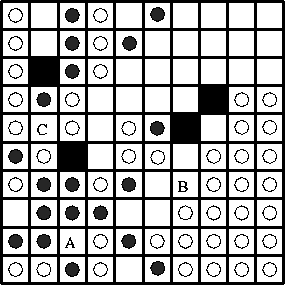
\includegraphics[scale=0.50]{stability.PNG}\\
Stable positions for white
\end{center}

Stability is a relatively expensive check because determining the stability of one piece requires testing a considerable number of points along the board. Complete board checking requires testing every single nonempty position. Additionally, since piece stability can depend on nearby pieces, to accurately find all stable positions we need to loop through the entire board until we find no new stable positions. This checking greatly slows down the search speeds, which became an issue due to the time constraints of the problem.

Stability memory was implemented in order to decrease the cost of computing stable nodes. Exploiting the fact that once a position is stable, it is always stable, we can keep track of the pieces that have already been found to be stable, and update this as we move. This avoids the need to repeatedly do an expensive complete board stability check. While overall this requires more computation from root game tree node to leaf, it moves the computation up as far in the game tree as possible, so that the computation is done once and shared along all the branches rather than being fully computed at each leaf node.

At the start of every move decision, the root node's complete board stability is checked. As each possible move is expanded, the stability of that move is checked. If that move fills any directional axes, the directional axes that were filled are checked. The results are saved in a stability matrix, and passed down the game tree. This greatly reduces total computation required.

It should be noted that this method is not complete, only a largely accurate estimate. There are less common circumstances where this algorithm gives false negatives. If a piece is made stable only by the stability of a point along the axis, it may not be found to be stable.

To fix this, we could test all pieces in all directions of a move, and then if we find any stable positions, retest all the directions from the stable positions. However, the increased computation required would outweigh the benefits of the gain in accuracy.

\begin{center}
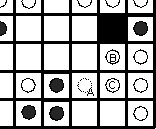
\includegraphics[scale=0.6]{falsepos.PNG}\\
If white moves in position A, the algorithm will detect that B is stable\\ but will fail to test the stability of C as it is not on a full line.
\end{center}

    \begin{itemize}
  \item
    Importance gets diluted in late game because in late game, EVERYTHING is stable. this is a consequence of only using 3 phases
  \end{itemize}

\section*{\emph{\textmd{Mobility}}}
\hrule

Mobility is the number of moves a player has in a given board state. High mobility increases the number of options available to a player, increasing the change they have a good move, and that they can out-position their opponent. Low mobility can reflect a poor position with a lack of options, and lead to forced moves.

Mobility tends to be the strongest predictor of a good position during the early game. In the mid and late game, it is less favoured than stability and control of the corners, but otherwise is still a strong predictor of the value of a position.

It also has the unfortunate side effect of increasing the branching factor in the MinMax search, to the point where the increased number of available moves can mean we have to search to a lesser depth.

\section*{\emph{\textmd{Piece Internality}}}
\hrule

A piece is internal if it has no empty neighbours. This can be a useful indicator of a player's position as it increases their maneuverability in the early and mid game as the middle becomes mostly full and possible moves are expansions to the outer edges. Internal pieces can also be harder to dislodge.

This is computationally cheap to check. Exploiting the fact internal pieces stay internal even if they are flipped, partial memory of internality was also used (internality checked and remembered for every new move).

\begin{center}
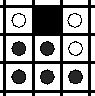
\includegraphics[scale=0.50]{internality.PNG}\\
The centre piece is an internal node.
\end{center}

\section*{\emph{Temporal Difference Learning}}
\hrule

Our learning algorithm is based on TD($\lambda$), although we do not implement that algorithm exactly.

When learning is enabled, we play through the entirity of a game, storing each board position. At the end, we recieve a reward equal to the difference in the number of pieces for each player in the terminal state.

Then, for each board $b_k$, and for each feature weight $W_f$, we choose which direction to adjust the weight in by making a small change in the value of the weight, and determining whether that would improve or worsen the value of the board. The point here is that we are calculating an approximation of the gradient of our evaluation function $V(b)$ at $b_k$, with respect to the feature $W_f$: $\frac{\Delta V(b_k)}{\Delta W_f}$, thus allowing us to perform gradient descent.

We then run through each successor $b_t$ of $b_k$, and calculate the difference between the value of $b_t$ and $b_k$, weighted by some discount factor $\gamma^{t-k}$.

Finally, the value of the feedback is also added in, weighted by the distance from $b_k$ to the terminal board $b_K$.

More formally, we calculate 
\[
	W_f \leftarrow W_f 
	+ \alpha \frac{\Delta V(b_k)}{\Delta W_f} \left(\gamma^{K-k}r + \sum_{t=k+1}^K \gamma^{t-k}\left(V(b_t) - V(b_k)\right)\right)
\]

Where
   \begin{itemize}
  \item
  	$W_f$ is the weight of feature $f$,
  \item
	$V(b_i)$ is the value of a board $b_i$,
  \item
	$r$ is our reward,
 \item
	$\alpha$ is our learning rate,
  \item
	$\gamma$ is our discount factor, and
  \item
	$K$ is the index of the terminal board.
  \end{itemize}

Values of $alpha = 0.0001$ and $\gamma = 0.9$ were used during our learning process.

To try and balance the exploration vs exploitation problem that is so frequently found in temporal difference learning, we utilised an $\epsilon$-greedy policy, whereby the agent would select a random move 15\% of the time, and an optimal (in the sense of its estimate of the value of a board state) move 85\% of the time.

\section*{\emph{Negamax with alpha beta pruning}}
\hrule

Negamax is an adversarial search algorithm which expands the game tree in a depth first search in order to maximise game value, under the assumption that the opponent, who makes the same assumptions about game value, is trying to minimise that value. This is achieved in a simple recursive fashion by recursively calling negamax and negating the values at each step.

The alpha-beta pruning extension allows us to disregard branches of the game tree that a player would not give the opponent a chance to play (because it is too good for their opponent), significantly reducing the size of the game tree that needs exploring.

Negamax is very useful as it emulates a game play environment, where while we moving the board into a good state for us, the opponent is actively trying to move to make the board a worse state for us.

The major disadvantage of Negamax is the assumption that the opponent values each board exactly the same way as we do. This is especially problematic with alpha beta pruning - we may prune states which very good moves based on the assumption that the opponent will never let us play those moves, but in real play, the opponent might let us play those moves if they don't see the value.

\section*{\emph{\textmd{Negamax Implementation}}}
\hrule

Because the entire game tree isn't computable, our negamax has a depth cutoff. A small (but useful) optimisation to this process is increasing the search depth by 1 if we explore along a forced move - both because there is no branching that would increase computation cost, and this is an interesting board that we should explore further.

At the cutoff, the agent uses the static evaluation function in order to determine how far in our favour a board state is.

At terminal states, the board is evaluated to be -$\infty$ if we lose, or +$\infty$ if we win. This encodes the fact that any win is equal, regardless of the piece margin, and we should prioritise an outright win, and also that any loss is equal and should be avoided at all costs.

The advantages are that we will take a guaranteed opportunity to wipe out the opponent early, or at the end of the game, move towards a safe guaranteed win rather than trying for a win with the most pieces. However the disadvantage is if we see that a perfect opponent would cause us to lose no matter how well we play, the agent surrenders and plays the first move it sees, rather than attempting to minimise the loss margin in the hope that the opponent makes a mistake and allows our victory.

In normal play, the agent searched to a depth of 7 in the game tree (see Time Management). Once the end of the game was within sight (12 moves left on the board), the depth was increased to allow the entire game tree to be evaluated. This allowed us to make perfect play (and at this point, we could determine whether we would win or lose to a perfect player).

\section*{\emph{Concurrency}}
\hrule

We utilised concurrency to reduce the amount of time taken to do a MinMax search to a fixed depth. This involved splitting the workload of computing the search tree between a number of worker tasks, typically equal to the number of CPU cores available to use for computation.

In doing so, we had to find a model of parallelism which balanced what was theoretically an optimal way of parallelising the computation, with the reality that any model of parallelism involves at least some overhead in communication between tasks, and in waiting on access to shared data structures.

The first model considered was one in which the root node of the MinMax search tree is pushed onto a stack, and then the worker nodes pop from this stack, expand the node which they popped, and push the resulting list back onto the stack. The result would be an approximately-depth-first search, and is \begin{em} theoretically \end{em} a very nice model of parallelism, since worker time is assigned where it is actually needed. However, there is the potential for significant overhead in writing to the stack (especially as Ada has a habit of copying variables instead of referencing them), leading to long waiting times for accessing it. There is also a not inconsiderable amount of overhead involved in tracking alpha-beta values and the best values for particular moves, which would make implementing this model challenging.

We therefore settled on a second, more straightforward method of parallelising the computation. In this model, the worker threads poll a central data structure in order to recieve a node to evaluate. This node corresponds to one of the Min nodes which are direct successors of the root Max node in the MinMax search tree. The node is then evaluated in full (to the specified fixed depth) and without communication with either the other workers or the central data structure. Once evaluated, the results (i.e the value of that move) are reported to the central data structure, which aggregates the results. The worker then requests a new node to evaluate, and the process repeats.

\begin{center}
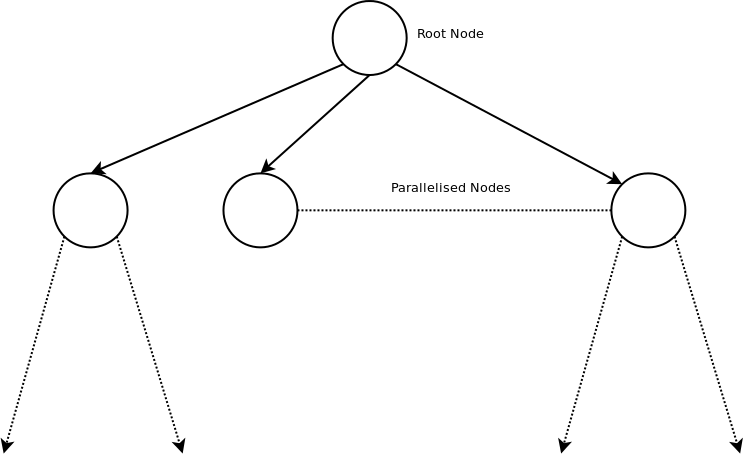
\includegraphics[scale=0.35]{concurrency.png}
\\Concurrency model
\end{center}

This model has the advantage of having very little overhead in terms of communication, and a relatively low chance of two worker tasks trying to simultaneously access the data structure (at least after the first batch of nodes is given out). The downside is that there is no consideration given to the amount of resources (i.e. worker time) needed to evaluate a node - the same amount of resources are allocated regardless of whether the node is a terminal, or a full search tree with a large branching factor. In practice however, this is not a significant problem, as if one node is evaluated quickly, the worker will simply be assigned another one.

One issue that does arise with this model is that the first node (or first set of nodes) evaluated almost always takes the longest amount of time, when compared with the other nodes. This appears to be true regardless of the number of workers assigned to the task. Our theory as to the reason behind this is that, for the first nodes, we do not have accurate $\alpha\beta$ values when exploring the tree, so much more will tend to be explored than is strictly necessary. Once at least one of the initial nodes returns, and its information aggreated into the central data structure, all subsequent nodes will be evaluated with at least the $\alpha\beta$ values of that first node, allowing for much more efficient pruning.

The results of our parallelism is an $O(n)$ speed-up in computation time, where $n$ is the number of cores we are using. In practice, this gave us an extra one to two levels of MinMax search, running on a 4-core machine.

\section*{\emph{Time management}}
\hrule
    \begin{itemize}
  \item
    Vary the search depth depending on time left and how long the previous move took
  \item
     Below 5 seconds, drop to depth 2  
  \item
    Below 15 seconds, drop to depth 4
  \item
    If we have extra time, increase to 8
  \item
    If we have less time, decrease to 5
  \item
    Default to 7
  \end{itemize}

\section*{\emph{C++ and Ada}}
\hrule
The main function in C++ was used to facilitate network communications, from the sample client code. C++ then called the appropriate functions in Ada to 
    \begin{itemize}
  \item
    We took the C++ sample client code and used it to call procedures in Ada
  \item
    C++ client listened for new messages and saved them
  \item
   C++ called Ada procedures
  \item
   Procedures called entries on Ada's Main Task
  \item
   Messages and information passed using direct edits to shared memory
  \end{itemize}

\section*{\emph{\textmd{C++ and Ada Experiences}}}
\hrule
    \begin{itemize}
  \item
    Make the communication as simple as possible
  \item
   Don't call entries or complex data structures
  \item
   C++ decapitalises everything
  \item
   Avoid C++ and Ada running computation concurrently near shared data
  \item
   C++ and Ada store arrays in different fashions
  \end{itemize}

\section*{\emph{Other ideas (Monte Carlo)}}
\hrule
    \begin{itemize}
  \item
    	Use monte carlo prediction as a substitute for reward to help with learning of mid-game states
  \item
	Tends to make the algorithm learn more quickly, and on-the-fly
  \item
	Can also be used as a predictor of how good a board state is.
  \end{itemize}

\section*{\emph{Other ideas (MinMax)}}
\hrule
    \begin{itemize}
  \item
    Optimised search ordering - expand nodes by their value in our piece feature weights
  \item
	Store searches between moves. Could have saved a huge amount of computation time.
  \item
	Vary depth of search based on branching factor and volatility of the state.
  \end{itemize}

\section*{\emph{Other ideas (Evolutionary Algorithm)}}
\hrule
    \begin{itemize}
  \item
   	Use an evolutionary algorithm strategy to play agents off against each other.
  \item
	Use feature values as 'genes'.
  \item
	'Breeding' via exchanging features. Don't need a heuristic for which to exchange, as features tend to be relatively independent.
  \item
	Mutation via small random change to a feature.
	\\ e.g. from a uniform distribution around (-1,1), or
	\\ Normal distribution with mean 0.
  \item
	Essentially still doing gradient decent. Can be used as a substitute for an $\epsilon$-greedy policy.
  \end{itemize}

\section*{\emph{Other ideas (Utilising opponent time)}}
\hrule
    \begin{itemize}
  \item
   	Compute further down the game tree while the opponent is thinking
  \item
	Could allow significantly greater search depths to be reached
  \item
	Required memory management and large data structures
  \item
	Ada would be very well positioned to perform this task
  \end{itemize}

\end{multicols}
\end{document} 
